\section{Experimental Setup}
\label{sec:setup}
\textbf{Code, checkpoints and data.} We use the official HazyResearch/ncm repository~\citep{kumbong2026ncm} without modification, the released \texttt{generator.pt}/\texttt{tokenizer.pt} pairs for Sudoku (easy, medium, hard; 25.6M-parameter generator, 15.0M-parameter tokenizer, 12 levels $[1,2,4,6,9,13,18,26,37,50,67,89]$, codebook size 16), WMT14 De--En~\citep{bojar2014wmt} (11 levels, Qwen3 pre-tokenizer) and XSum~\citep{narayan2018xsum} (9 levels $[4,6,10,14,20,26,32,40,48]$, GPT-2 pre-tokenizer, prefix length 512), and the corresponding files of \texttt{hazyresearch/ncm-datasets}. Our evaluation focuses on conditional generation and constraint-satisfaction tasks with ground-truth references, where exact-match and reference-based fidelity can be computed deterministically, without the variance of an external language-model judge such as the GPT-2 Large perplexity used for unconditional TinyStories~\citep{eldan2023tinystories} generation.

\textbf{Splits.} The released data contain only test files for these tasks (the XSum file \texttt{validation\_cond512\_le48.pickle} is not part of the public dataset repository). We therefore split each official test file deterministically: the first 500 Sudoku boards (per difficulty), 1{,}000 WMT14 sentences and 500 XSum articles are used to train $C_\omega$ and select all hyper-parameters (Section~\ref{sec:select}); results are reported on the next 1{,}500 boards, the remaining 2{,}003 sentences and the next 1{,}000 articles. Zero-shot halting curves (no learned component) additionally use all 2{,}000 Sudoku boards.

\textbf{Baseline reproduction.} The official evaluator was run as \texttt{python evaluate.py --config config/eval/<task>.yaml --checkpoint-dir <ck> --data-dir <data> --out <dir> --gpus 0}. It gives \OffEasy/\OffMedium/\OffHard\% solved boards on the full Sudoku test sets, \OffWmt{} BLEU on WMT14 (3{,}003 sentences) and R-1/R-2/R-L $=$ \OffXsumRone/\OffXsumRtwo/\OffXsumRL{} on the first 1{,}500 XSum articles; these agree with the numbers reported for the released checkpoints~\citep{kumbong2026ncm}. Our wrapped sampler reproduces the official latents bit-exactly (Appendix~\ref{app:repro}); on our test portions NCM scores \BaseEasy/\BaseMedium/\BaseHard\% (Sudoku), \BaseWmt{} BLEU and \BaseXsum{} R-L.

\textbf{Hardware and profiling.} Every number comes from Kaggle Tesla T4 (16\,GB, 14.6\,GB usable) sessions with Python 3.13 and the preinstalled PyTorch~\citep{paszke2019pytorch} CUDA build. Wall-clock latency is the mean over evaluation batches after one untimed warm-up batch, synchronized with \texttt{torch.cuda.synchronize}; peak memory is \texttt{torch.cuda.max\_memory\_allocated}. Variants of the same task were timed in the same session. Hyper-parameters are listed in Table~\ref{tab:hp}.

\begin{table}[t]
\centering
\caption{Hyper-parameters. Generator and tokenizer settings are those of the official evaluation configs.}
\label{tab:hp}
\footnotesize\setlength{\tabcolsep}{2.5pt}
\begin{tabular}{lccc}
\toprule
 & Sudoku & WMT14 & XSum\\
\midrule
levels $K$ & 12 & 11 & 9\\
$L$, $d$ & 89, 256 & 64, 768 & 48, 768\\
generator params & 25.5M & 120.0M & 88.0M\\
$C_\omega$ params (width) & 1.23M & 1.20M & 1.20M\\
train / test items & 500 / 1500 & 1000 / 2003 & 500 / 1000\\
epochs & 40 & 20 & 30\\
batch (train / eval) & 32 / 128 & 32 / 64 & 32 / 32\\
optimizer & \multicolumn{3}{c}{AdamW~\citep{loshchilov2019adamw}, lr $3{\times}10^{-4}$, wd 0.01, one-cycle, clip 1.0}\\
$\alpha$ (KL weight) & \multicolumn{3}{c}{0.1}\\
$\eta_k$ init / scale grid & \multicolumn{3}{c}{$\sigma(\beta_k)=0.5$ / $s\in\{0,0.25,0.5,1\}$}\\
rollout / corruption mix & \multicolumn{3}{c}{0.75 / 0.25 (2 corrupted copies, $u\sim\mathcal{U}(0,1)$)}\\
$\tau$ grid, $k_{\min}$ & \multicolumn{3}{c}{\{0.01,0.03,0.05,0.10,0.15\}, 2}\\
$\tau_{\mathrm{tok}}$ grid & \multicolumn{3}{c}{\{0.005,0.01,0.02,0.05\}}\\
selection tolerance & \multicolumn{3}{c}{0.5 points of full-depth quality}\\
seeds & \multicolumn{3}{c}{42, 0, 1, 2, 3}\\
\bottomrule
\end{tabular}
\end{table}


\textbf{Runs.} We report three corrector configurations, each with five seeds: (i) \emph{in-loop, no selection}: the final-epoch corrector with learned $\eta_k$ is applied in the generation loop; (ii) \emph{in-loop, validation-selected}: best-validation checkpoint and closed-loop step-size scale $s$ (Section~\ref{sec:select}); (iii) \emph{decode-path}: as (ii) but the corrector acts only on decoded latents, with per-level $s_k$. Halting-only uses uncorrected latents and the rule and $\tau$ selected on the training portion; ``$C_\omega$+halt'' re-selects the rule and $\tau$ with the corrector in place. Configuration (ii) was not run on XSum.

\section{Results and Ablations}
\label{sec:results}
\begin{table*}[t]
\centering
\caption{Main comparison on official NCM checkpoints (single Tesla T4). Quality: Sudoku boards solved (\%), WMT14 corpus BLEU, XSum ROUGE-L, on held-out test items (Sudoku 1{,}500, WMT14 2{,}003, XSum 1{,}000). Learned rows: mean$\pm$std over seeds \{42,0,1,2,3\}. $\bar k$: mean levels executed. GFLOPs: per evaluation batch, measured. ms: wall-clock per batch (Sudoku 128, WMT14 64, XSum 32 sequences). MB: peak allocated GPU memory. $p_W$: smallest paired Wilcoxon $p$ over seeds vs.\ NCM (per-item cell acc./sentence BLEU/ROUGE-L). $p_2$: smallest exact McNemar $p$ on solved boards (Sudoku) or one-sample $t$-test of seed means (text). ``no sel.'': trained without validation checkpoint and step-size selection.}
\label{tab:main}
\setlength{\tabcolsep}{3.2pt}
\begin{tabular}{llccccccc}
\toprule
 & Method & Quality & $\bar k$ & GFLOPs & ms & MB & $p_W$ & $p_2$\\
\midrule
\multirow{8}{*}{\rotatebox{90}{\scriptsize Sudoku-easy}} & NCM (official) & 99.47 & 12.0 & 74.7 & 3426 & 3821 & -- & --\\
 & + halting & 99.47 & 12.0 & 74.7 & 3485 & 4030 & 1.0 & --\\
 & $C_\omega$ (in-loop, no sel.) & 58.17$\pm$9.05 & 12.00 & 77.2 & 3639 & 4091 & $<$$10^{-4}$ & $<$$10^{-4}$\\
 & $C_\omega$+halt (in-loop, no sel.) & 58.17$\pm$9.05 & 12.00 & 77.2 & 3634 & 5595 & $<$$10^{-4}$ & $<$$10^{-4}$\\
 & $C_\omega$ (in-loop, val.-sel.) & 99.47$\pm$0.00 & 12.00 & 77.2 & 3678 & 4231 & 0.059 & 1.0\\
 & $C_\omega$+halt (in-loop, val.-sel.) & 99.47$\pm$0.00 & 12.00 & 77.2 & 3697 & 5464 & 0.059 & 1.0\\
 & $C_\omega$ (decode-path) & 99.47$\pm$0.00 & 12.00 & 77.5 & 4314 & 4685 & 1.0 & 1.0\\
 & $C_\omega$+halt (decode-path) & 99.47$\pm$0.00 & 12.00 & 77.5 & 4315 & 5074 & 1.0 & 1.0\\
\midrule
\multirow{8}{*}{\rotatebox{90}{\scriptsize Sudoku-medium}} & NCM (official) & 96.00 & 12.0 & 74.7 & 3436 & 3821 & -- & --\\
 & + halting & 96.00 & 12.0 & 74.7 & 3482 & 4029 & 1.0 & --\\
 & $C_\omega$ (in-loop, no sel.) & 78.03$\pm$5.52 & 12.00 & 77.2 & 3634 & 4094 & $<$$10^{-4}$ & $<$$10^{-4}$\\
 & $C_\omega$+halt (in-loop, no sel.) & 78.03$\pm$5.52 & 12.00 & 77.2 & 3630 & 5598 & $<$$10^{-4}$ & $<$$10^{-4}$\\
 & $C_\omega$ (in-loop, val.-sel.) & 96.00$\pm$0.00 & 12.00 & 77.2 & 3684 & 4960 & 1.0 & 1.0\\
 & $C_\omega$+halt (in-loop, val.-sel.) & 96.00$\pm$0.00 & 12.00 & 77.2 & 3686 & 4490 & 1.0 & 1.0\\
 & $C_\omega$ (decode-path) & 96.00$\pm$0.00 & 12.00 & 77.5 & 3903 & 4551 & 1.0 & 1.0\\
 & $C_\omega$+halt (decode-path) & 96.00$\pm$0.00 & 12.00 & 77.5 & 3902 & 5181 & 1.0 & 1.0\\
\midrule
\multirow{8}{*}{\rotatebox{90}{\scriptsize Sudoku-hard}} & NCM (official) & 86.67 & 12.0 & 74.7 & 3436 & 3821 & -- & --\\
 & + halting & 86.67 & 12.0 & 74.7 & 3481 & 3837 & 1.0 & --\\
 & $C_\omega$ (in-loop, no sel.) & 24.19$\pm$11.72 & 12.00 & 77.2 & 3637 & 5090 & $<$$10^{-4}$ & $<$$10^{-4}$\\
 & $C_\omega$+halt (in-loop, no sel.) & 24.19$\pm$11.72 & 12.00 & 77.2 & 3631 & 4053 & $<$$10^{-4}$ & $<$$10^{-4}$\\
 & $C_\omega$ (in-loop, val.-sel.) & 86.79$\pm$0.17 & 12.00 & 77.2 & 3679 & 5323 & 0.221 & 0.454\\
 & $C_\omega$+halt (in-loop, val.-sel.) & 86.79$\pm$0.17 & 12.00 & 77.2 & 3697 & 4085 & 0.221 & 0.454\\
 & $C_\omega$ (decode-path) & 86.67$\pm$0.00 & 12.00 & 77.5 & 3915 & 4644 & 1.0 & 1.0\\
 & $C_\omega$+halt (decode-path) & 86.67$\pm$0.00 & 12.00 & 77.5 & 3908 & 4660 & 1.0 & 1.0\\
\midrule
\multirow{8}{*}{\rotatebox{90}{\scriptsize WMT14 De--En}} & NCM (official) & 22.35 & 11.0 & 249.4 & 6204 & 8196 & -- & --\\
 & + halting & 22.35 & 11.0 & 249.4 & 6196 & 7106 & 1.0 & --\\
 & $C_\omega$ (in-loop, no sel.) & 0.21$\pm$0.10 & 11.00 & 251.1 & 6260 & 8144 & $<$$10^{-4}$ & $<$$10^{-4}$\\
 & $C_\omega$+halt (in-loop, no sel.) & 0.09$\pm$0.08 & 10.66 & 251.1 & 8562 & 7281 & $<$$10^{-4}$ & $<$$10^{-4}$\\
 & $C_\omega$ (in-loop, val.-sel.) & 22.35$\pm$0.00 & 11.00 & 251.1 & 6203 & 8144 & 1.0 & 1.0\\
 & $C_\omega$+halt (in-loop, val.-sel.) & 22.35$\pm$0.00 & 11.00 & 251.1 & 6216 & 7139 & 1.0 & 1.0\\
 & $C_\omega$ (decode-path) & 22.35$\pm$0.00 & 11.00 & 251.3 & 6024 & 8038 & 1.0 & 1.0\\
 & $C_\omega$+halt (decode-path) & 22.35$\pm$0.00 & 11.00 & 251.3 & 6025 & 7274 & 1.0 & 1.0\\
\midrule
\multirow{6}{*}{\rotatebox{90}{\scriptsize XSum}} & NCM (official) & 27.62 & 9.0 & 915.1 & 10324 & 5692 & -- & --\\
 & + halting & 27.62 & 9.0 & 915.1 & 10303 & 7051 & 1.0 & --\\
 & $C_\omega$ (in-loop, no sel.) & 6.25$\pm$0.12 & 9.00 & 918.3 & 10329 & 7080 & $<$$10^{-4}$ & $<$$10^{-4}$\\
 & $C_\omega$+halt (in-loop, no sel.) & 6.19$\pm$0.13 & 8.94 & 918.3 & 10477 & 7044 & $<$$10^{-4}$ & $<$$10^{-4}$\\
 & $C_\omega$ (decode-path) & 27.62$\pm$0.00 & 9.00 & 918.7 & 11839 & 7498 & 1.0 & 1.0\\
 & $C_\omega$+halt (decode-path) & 27.62$\pm$0.00 & 9.00 & 918.7 & 11862 & 6921 & 1.0 & 1.0\\
\bottomrule
\end{tabular}
\end{table*}


\subsection{Main comparison}
Table~\ref{tab:main} gives the four-way comparison. Three findings hold across all tasks.

\textit{Halting does not trigger at matched quality.} On every task, the rule and $\tau$ selected on the training portion run all $K$ levels, so halting-only coincides with NCM in quality and FLOPs and is marginally slower because of the criterion evaluation. Earlier termination is possible only by accepting large losses (Section~\ref{sec:halt}).

\textit{In-loop correction without selection is harmful.} Feeding the corrected latent back to the generator reduces Sudoku-hard solved boards from \BaseHard\% to \LoopVoneHard\% (5-seed mean), WMT14 from \BaseWmt{} to \LoopVoneWmt{} BLEU and XSum from \BaseXsum{} to \LoopVoneXsum{} R-L; all differences have McNemar or Wilcoxon $p<10^{-4}$. This happens although the open-loop validation MSE of the corrector is lower than that of the uncorrected latent (e.g.\ on WMT14, the epoch-20 rollout MSE is 0.90--1.00 versus 1.19--1.37 without correction).

\textit{With selection, the corrector reduces to (near) identity.} When the step-size scale is chosen by closed-loop validation quality, it is $s=0$ for all five seeds on WMT14 and Sudoku-medium, four of five on Sudoku-easy and three of five on Sudoku-hard; with $s=0$ the corrected sampler is identical to NCM. The largest remaining effect is on Sudoku-hard, \LoopVtwoHard$\pm$\LoopVtwoHardStd\% versus \BaseHard\% solved, which is not significant (smallest McNemar $p=\LoopVtwoHardP$, $t$-test $p=\LoopVtwoHardT$). The decode-path corrector leaves the final level unchanged on every evaluated task because the validation-selected scale at the last level is $0$ for every seed. Both corrected variants cost up to 26\% additional latency and 0.3--3.7\% additional FLOPs.

\begin{figure}[t]
\centering
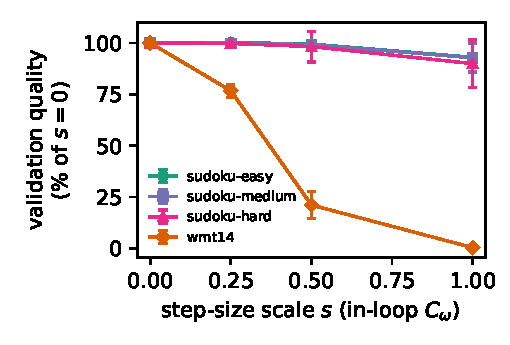
\includegraphics[width=\columnwidth]{figs/fig_dose.pdf}
\caption{Closed-loop validation quality of the in-loop corrector as a function of its step-size scale $s$ (relative to $s=0$, mean$\pm$std over five seeds; Sudoku: solve rate, WMT14: BLEU). Quality decreases monotonically with $s$; the effect is strongest for translation, where the generator is most sensitive to its input latent.}
\label{fig:dose}
\end{figure}

\subsection{Why in-loop correction fails: exposure to off-distribution inputs}
Figure~\ref{fig:dose} shows the closed-loop dose-response: validation quality decreases monotonically with the step-size scale. On WMT14 it drops to roughly three quarters of the baseline at $s=0.25$ and to almost zero at $s=1$. The open-loop objective~\eqref{eq:loss} rewards moving $\zh^{(k)}$ towards $\zh^{(k)}_{\mathrm{GT}}$ \emph{on average}, but the generator was trained only on inputs $u_{k+1}$ obtained from exact cumulative sums of codewords (clean or corrupted). A corrected latent is a continuous point that is closer in $\ell_2$ yet not of this form, and the generator's code predictions on such inputs are much worse. This is the exposure-bias mechanism~\citep{bengio2015scheduled,ross2011dagger}, and it is the failure mode anticipated in the caveat to Proposition~\ref{prop:contraction}: the bound holds at the error rate $\sigma_k$ of the \emph{corrected} process, which is far above that of NCM.

\textbf{On-manifold projection.} If exposure to non-lattice inputs is the cause, projecting the corrected latent back onto the lattice of codeword sums should remove most of the collapse. After applying $C_\omega$ at level $k$, we re-quantize the level-$k$ residual against $\mathcal{V}_k$, $\tilde r_k=\arg\min_v\|\mathrm{Down}_k(\zt^{(k)}-\zh^{(k-1)})-e_{k,v}\|_2$, and feed $\zh^{(k-1)}+\Phi_k(\Up_k(E_k(\tilde r_k)))$ to the generator, so every input is again a sum $\sum_{j\le k}\Phi_j\Up_jE_j(\cdot)$. On a 32-board Sudoku-hard check set (seed-42 correctors), projection raises the unselected in-loop corrector from \ProjNoSelOff\% to \ProjNoSelOn\% solved, against \ProjNCM\% for untouched NCM; for the validation-selected corrector it gives \ProjSelOn\% (\ProjSelOff\% without projection). This confirms the exposure-bias diagnosis. Projection still trails NCM because nearest-neighbor re-quantization of one level cannot recover the global constraint satisfaction that the generator's own codes encode.

\textbf{Closed-loop co-adaptation of the generator.} The remaining option is to adapt the generator to revised trajectories. Table~\ref{tab:dagger} fine-tunes the generator on the 400 training boards with teacher-forced reference states (control), with DAgger~\citep{ross2011dagger} on a 50/50 mix of reference and on-policy rollout states labelled by greedy residual quantization of $z-\text{state}$, and with DAgger plus a jointly trained in-loop $C_\omega$. No arm beats NCM. On Sudoku-hard the three arms reach \DgTfHard, \DgDagHard{} and \DgDagCHard\% (NCM \BaseHard\%; seed-mean $t$-test $p=\DgPTfHard$, $\DgPDagHard$, $\DgPDagCHard$), and on Sudoku-medium \DgTfMedium, \DgDagMedium{} and \DgDagCMedium\% (NCM 96.00\%). On Sudoku-easy all three arms are significantly \emph{worse} (\DgTfEasy, \DgDagEasy, \DgDagCEasy\% vs.\ 99.47\%, $p\le\DgPTfEasy$), because the 100-board validation set is saturated and cannot distinguish checkpoints. Validation accuracy decreases during fine-tuning on Sudoku-hard, and selection keeps the official model for one to three of five seeds on hard and medium. A few hundred boards cannot move the decision boundaries of a 25M-parameter generator that was fitted jointly with fixed codebooks during large-scale Stage-2 training; small-sample closed-loop adaptation overfits before it removes the shift.

\begin{table*}[t]
\centering
\caption{Closed-loop co-adaptation of the generator on Sudoku (1{,}500 held-out boards; 5 seeds). All arms fine-tune the 25.3M non-embedding generator parameters on the 400 training boards of $N_{\mathrm{tr}}$ for 3 rounds $\times$ 4 epochs (AdamW, lr $3{\times}10^{-5}$) and select the checkpoint by closed-loop solve rate on the 100 validation boards (the official model is a candidate). \emph{Control}: teacher-forced reference states. \emph{DAgger}: 50/50 reference and on-policy rollout states, labels given by greedy residual quantization of $z-\text{state}$. \emph{DAgger}+$C_\omega$: rollout states revised by a jointly trained in-loop corrector. Cells: solved \% mean$\pm$std (seed-mean $t$-test $p$ vs.\ NCM; number of seeds for which the official model was selected).}
\label{tab:dagger}
\setlength{\tabcolsep}{4pt}
\begin{tabular}{lcccc}
\toprule
 & NCM & Control (TF fine-tune) & DAgger & DAgger + $C_\omega$\\
\midrule
Sudoku-easy & 99.47 & 98.96$\pm$0.15 (0.002; 0/5) & 98.92$\pm$0.12 (5.1e-04; 0/5) & 99.04$\pm$0.14 (0.002; 0/5)\\
Sudoku-medium & 96.00 & 95.93$\pm$0.12 (0.266; 3/5) & 95.75$\pm$0.43 (0.261; 3/5) & 95.75$\pm$0.33 (0.162; 2/5)\\
Sudoku-hard & 86.67 & 85.87$\pm$1.10 (0.178; 3/5) & 86.27$\pm$0.58 (0.197; 2/5) & 86.27$\pm$0.96 (0.404; 1/5)\\
\bottomrule
\end{tabular}
\end{table*}


\begin{table*}[t]
\centering
\caption{Quality of the decoded intermediate latent $D_\psi(\zh^{(k)})$ (or $D_\psi(\zt^{(k)})$) at every level $k$, seed 42, test items. Fine-drop makes every level decodable, but quality rises steeply only over the last third of the hierarchy. WMT14 has 11 levels and XSum 9.}
\label{tab:levels}
\setlength{\tabcolsep}{2.6pt}
\begin{tabular}{llcccccccccccc}
\toprule
 & & \multicolumn{12}{c}{level $k$}\\
 & & 1 & 2 & 3 & 4 & 5 & 6 & 7 & 8 & 9 & 10 & 11 & 12\\
\midrule
Sudoku-hard cell acc. & NCM & 14.6 & 14.6 & 16.9 & 20.2 & 20.2 & 27.8 & 33.2 & 45.5 & 62.0 & 76.1 & 81.9 & 98.4\\
 & in-loop $C_\omega$ (no sel.) & 14.4 & 14.2 & 16.5 & 19.2 & 17.1 & 25.0 & 25.7 & 20.5 & 1.8 & 2.1 & 8.7 & 52.7\\
 & decode-path $C_\omega$ & 14.6 & 14.6 & 16.9 & 20.2 & 20.2 & 27.8 & 33.1 & 45.5 & 62.0 & 76.2 & 82.1 & 98.4\\
\midrule
Sudoku-hard solved & NCM & 0.0 & 0.0 & 0.0 & 0.0 & 0.0 & 0.0 & 0.0 & 0.0 & 0.0 & 0.0 & 0.0 & 86.7\\
 & in-loop $C_\omega$ (no sel.) & 0.0 & 0.0 & 0.0 & 0.0 & 0.0 & 0.0 & 0.0 & 0.0 & 0.0 & 0.0 & 0.0 & 17.9\\
 & decode-path $C_\omega$ & 0.0 & 0.0 & 0.0 & 0.0 & 0.0 & 0.0 & 0.0 & 0.0 & 0.0 & 0.0 & 0.0 & 86.7\\
\midrule
WMT14 BLEU & NCM & 0.4 & 0.9 & 1.6 & 2.9 & 5.0 & 7.6 & 12.3 & 15.4 & 17.7 & 19.2 & 22.3 & --\\
 & in-loop $C_\omega$ (no sel.) & 0.1 & 0.1 & 0.1 & 0.2 & 0.2 & 0.1 & 0.0 & 0.0 & 0.0 & 0.0 & 0.0 & --\\
 & decode-path $C_\omega$ & 0.4 & 0.9 & 1.5 & 2.8 & 5.0 & 7.6 & 12.3 & 15.4 & 17.7 & 19.2 & 22.3 & --\\
\midrule
XSum R-L & NCM & 19.2 & 21.7 & 23.0 & 23.6 & 24.5 & 25.4 & 26.1 & 26.4 & 27.6 & -- & -- & --\\
 & in-loop $C_\omega$ (no sel.) & 8.3 & 2.8 & 1.6 & 1.5 & 1.7 & 2.2 & 1.9 & 0.9 & 6.3 & -- & -- & --\\
 & decode-path $C_\omega$ & 19.2 & 21.7 & 23.0 & 23.6 & 24.5 & 25.4 & 26.1 & 26.4 & 27.6 & -- & -- & --\\
\bottomrule
\end{tabular}
\end{table*}


\subsection{Level-by-level decoding}
\label{sec:diag}
Table~\ref{tab:levels} and Figure~\ref{fig:levels} decode the latent after every level. Fine-drop training does make all levels decodable, but the information is concentrated in the last levels: on Sudoku-hard, cell accuracy is below 35\% up to level 7 (and no board is solved before the final level 12), and on WMT14 BLEU stays below 8 until level 6 and increases by more than 3 points at each of the last two levels. The decode-path corrector changes intermediate Sudoku cell accuracy by at most $0.57$ points (largest gains at levels 10--11 on Sudoku-easy and -medium, $\le0.22$ on Sudoku-hard) and lowers WMT14 BLEU by $0.10$--$0.13$ at levels 3--4, despite per-level scales selected on validation data. In-loop correction without selection lowers every level after the first few.

\begin{figure*}[t]
\centering
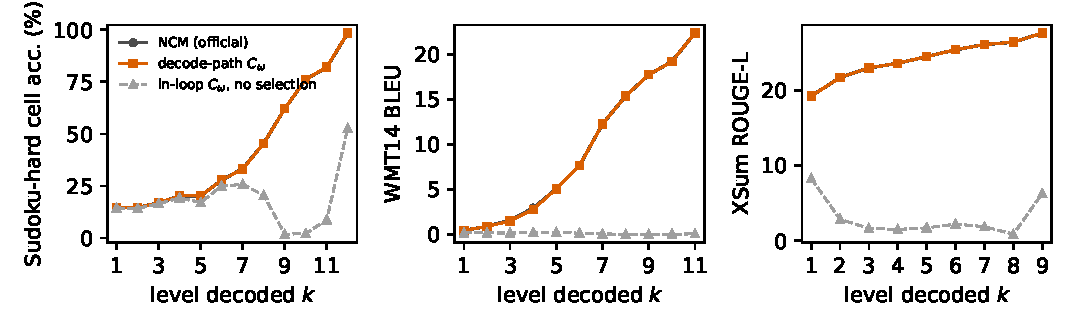
\includegraphics[width=\textwidth]{figs/fig_levels.pdf}
\caption{Quality of decoding at intermediate levels (seed 42, test items). Official NCM, decode-path corrector (overlapping NCM almost everywhere) and in-loop corrector without validation selection.}
\label{fig:levels}
\end{figure*}

\subsection{Halting trade-off}
\label{sec:halt}
Figure~\ref{fig:halt} and the top of Table~\ref{tab:sens} sweep $\tau$ on uncorrected latents. For small $\tau$ neither rule ever fires. When a rule does fire, it fires at an intermediate level whose decoding is poor: on all 2{,}000 Sudoku-hard boards the flux rule with $\tau=0.05$ stops after \ZsFluxFiveLevHard{} levels on average and solves \ZsFluxFiveHard\% (versus \ZsBaseHard\%), and the stability rule with $\tau=0.10$ stops after \ZsStabTenLevHard{} levels and solves \ZsStabTenHard\%. Figure~\ref{fig:flux} explains this behavior. The relative flux of the \emph{reference} latents is not monotone in $k$: on Sudoku-hard it drops to $0.045$ at level 5, where cell accuracy is only about 20\%, and rises again to above 0.4 at the fine levels. A threshold that lets the rule fire at all therefore fires at the coarse dip. On WMT14 the flux is never below 0.29. This is the empirical failure of Assumption~\ref{as:geo} quantified in Section~\ref{sec:theory}.

\begin{figure*}[t]
\centering
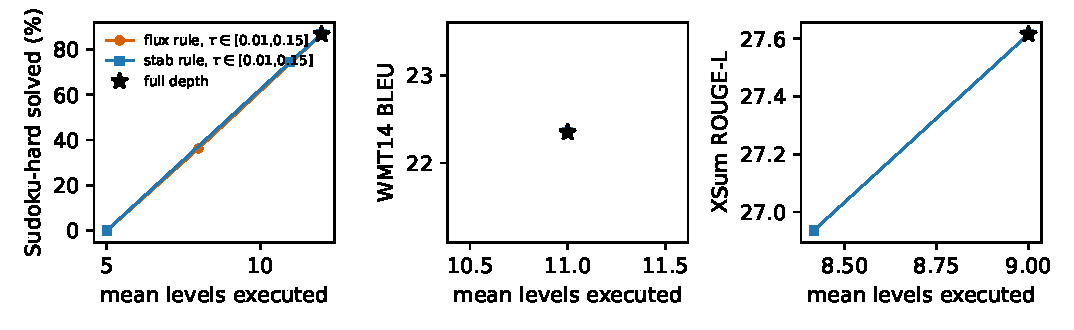
\includegraphics[width=\textwidth]{figs/fig_halt.pdf}
\caption{Quality versus mean executed levels for the flux and stability halting rules on uncorrected latents ($\tau\in\{0.01,\dots,0.15\}$, test items). Star: full depth. On WMT14 no setting halts; on XSum the stability rule at $\tau=0.15$ saves 0.6 levels on average at a cost of 0.7 ROUGE-L.}
\label{fig:halt}
\end{figure*}

\begin{figure}[t]
\centering
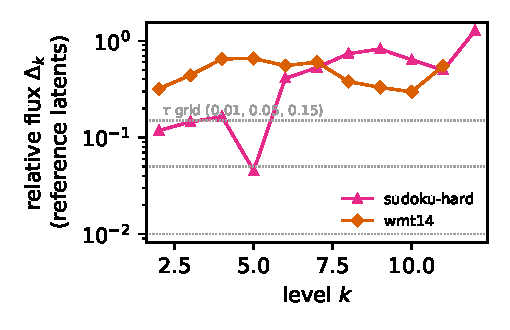
\includegraphics[width=\columnwidth]{figs/fig_flux.pdf}
\caption{Relative latent flux $\Delta_k$~\eqref{eq:flux} along reference trajectories of the released tokenizers (64 Sudoku-hard boards, 12 WMT14 sentences). Dotted lines mark the $\tau$ grid. The flux does not decay with $k$, which violates the premise of Proposition~\ref{prop:rd}.}
\label{fig:flux}
\end{figure}

\textbf{Token freezing.} At $\tau_{\mathrm{tok}}\le0.02$ fewer than 0.1\% of segments are ever frozen and outputs are unchanged. At $\tau_{\mathrm{tok}}=0.05$, 55\% of segments are frozen on Sudoku-hard and the solve rate drops from 86.7\% to 71.0\%; since freezing does not reduce FLOPs in the dense block-diagonal implementation, there is no setting with a favorable trade-off.

\begin{table}[t]
\centering
\caption{Sensitivity on Sudoku-hard (1{,}500 test boards; NCM: 86.7\% solved, 98.4\% cells). Top: halting threshold on uncorrected latents, cells give solved\,\% / $\bar k$ for the flux and stability rules. Middle and bottom: in-loop corrector with fixed $\eta_k$ (no step-size calibration) and different sizes (learned $\eta_k$, initialized at 0.5), seed 42, without and with validation checkpoint selection; columns give solved\,\%, cell\,\%, parameters, training time (s, 40 epochs on T4) and peak training memory (MB).}
\label{tab:sens}
\setlength{\tabcolsep}{2.4pt}
\begin{tabular}{lccccc}
\toprule
Setting & flux / solved & stab / cell & params & s & MB\\
\midrule
$\tau=0.01$ & 86.7 / 12.00 & 86.7 / 12.00 & -- & -- & --\\
$\tau=0.03$ & 86.7 / 12.00 & 86.7 / 12.00 & -- & -- & --\\
$\tau=0.05$ & 36.2 / 7.99 & 86.7 / 12.00 & -- & -- & --\\
$\tau=0.1$ & 0.0 / 5.00 & 74.4 / 10.97 & -- & -- & --\\
$\tau=0.15$ & 0.0 / 5.00 & 0.0 / 5.00 & -- & -- & --\\
\midrule
$\eta_k\equiv0.25$ (no sel.) & 17.4 & 52.5 & 1.23M & 127 & 3635\\
$\eta_k\equiv0.5$ (no sel.) & 10.5 & 41.7 & 1.23M & 127 & 3761\\
$\eta_k\equiv1.0$ (no sel.) & 44.3 & 73.8 & 1.23M & 127 & 2950\\
$\eta_k\equiv0.25$ (val.-sel.) & 86.4 & 98.3 & 1.23M & 122 & 1732\\
$\eta_k\equiv0.5$ (val.-sel.) & 86.5 & 98.4 & 1.23M & 122 & 1193\\
$\eta_k\equiv1.0$ (val.-sel.) & 86.4 & 98.4 & 1.23M & 122 & 820\\
\midrule
size 0.31M (no sel.) & 0.5 & 16.4 & 0.31M & 85 & 1560\\
size 1.23M (no sel.) & 17.9 & 52.7 & 1.23M & 127 & 3769\\
size 3.04M (no sel.) & 58.8 & 86.5 & 3.04M & 191 & 4360\\
size 0.31M (val.-sel.) & 62.5 & 89.3 & 0.31M & 82 & 813\\
size 1.23M (val.-sel.) & 86.5 & 98.4 & 1.23M & 122 & 812\\
size 3.04M (val.-sel.) & 86.9 & 98.4 & 3.04M & 181 & 834\\
\bottomrule
\end{tabular}
\end{table}


\textbf{Per-sequence margin halting with batch compaction.} Batch-lockstep halting forces the whole batch to wait for its hardest item, and raw flux has a coarse dip at level~5 (Fig.~\ref{fig:flux}). We therefore also implemented per-sequence halting with true batch compaction: each sequence halts individually for $k\ge8$ when its decoder top-1 margin $\mu_{i,k}=\min_t(p_{(1)}-p_{(2)})$ exceeds $\tau_{\mathrm{margin}}$ (Step~4 of Appendix~\ref{app:p2}) and its decoding is unchanged from level $k-1$, and halted sequences are removed from the active batch. The rule never fires for $\tau_{\mathrm{margin}}\in\{0.5,0.8,0.9,0.95\}$. Across 64 boards per difficulty, the share of boards whose level-$k$ decoding equals the final one is \MarginEqMax\% for every $k\le11$, between \FlipsMin{} and \FlipsMax{} cells still change at the last level, and the median margin at level~11 is at most \MarginMedMax. Task resolution is concentrated in the final level, so no lossless early exit exists for these checkpoints at any granularity.

\subsection{Sensitivity}
Table~\ref{tab:sens} varies the step size and the corrector size for the in-loop corrector on Sudoku-hard. Without validation selection, all configurations are far below NCM, and larger correctors are less harmful (0.31M: 0.5\%, 3.04M: 58.8\% solved). We attribute this to the zero-initialized output projection: a larger model fits the identity on rollout trajectories more closely. With validation checkpoint selection, the 1.23M and 3.04M correctors reach 86.4--86.9\% solved, within 0.2 points of NCM, while the 0.31M corrector reaches only 62.5\%. Training a 1.2M-parameter corrector for 40 epochs on 500 boards takes about two minutes on the T4 with at most 4.4\,GB peak memory (all sizes), and building the training trajectories takes 16\,s.

\begin{figure*}[t]\centering\scriptsize\setlength{\tabcolsep}{4pt}
\begin{tabular}{lcccc}
\toprule & level 3 & level 6 & level 9 & level 12\\\midrule
NCM & \texttt{\begin{tabular}{@{}c@{}}5 2 6 4 7 4 7 3 6\\3 7 1 3 7 1 2 9 6\\8 7 1 2 7 8 2 9 6\\2 3 7 8 2 6 1 7 6\\6 5 7 5 8 7 1 2 4\\2 4 7 9 2 6 8 6 4\\7 1 3 7 1 4 2 8 8\\7 8 3 7 3 4 6 7 9\\7 6 2 7 8 4 4 4 9\end{tabular}} & \texttt{\begin{tabular}{@{}c@{}}5 2 2 4 7 8 7 9 9\\9 9 9 4 3 3 2 3 2\\3 7 6 4 7 1 7 5 5\\5 5 5 5 8 7 8 7 4\\8 8 3 5 6 7 1 4 4\\4 4 4 9 2 6 3 3 3\\5 4 5 7 6 4 6 6 8\\6 6 6 7 8 5 4 5 5\\5 6 5 5 3 7 4 4 7\end{tabular}} & \texttt{\begin{tabular}{@{}c@{}}5 6 5 4 4 2 2 9 1\\1 7 9 8 6 5 5 2 2\\2 2 4 9 1 1 6 8 8\\7 5 6 9 1 4 3 3 2\\8 3 3 9 2 6 1 1 4\\4 1 1 1 3 7 9 5 5\\7 4 3 1 5 5 2 2 8\\9 1 1 6 8 3 5 4 4\\6 8 5 4 4 7 3 1 1\end{tabular}} & \texttt{\begin{tabular}{@{}c@{}}5 6 8 4 3 2 7 9 1\\9 7 1 8 6 5 4 2 3\\2 3 4 7 9 1 6 8 5\\7 5 6 9 1 4 8 3 2\\8 9 3 5 2 6 1 7 4\\4 1 2 3 7 8 9 5 6\\3 4 7 1 5 9 2 6 8\\1 2 9 6 8 3 5 4 7\\6 8 5 2 4 7 3 1 9\end{tabular}}\\\midrule
in-loop $C_\omega$ (no sel.) & \texttt{\begin{tabular}{@{}c@{}}5 2 2 4 4 4 4 8 8\\8 4 1 3 3 8 5 5 6\\8 7 6 2 7 8 2 4 6\\8 8 8 8 2 6 8 8 6\\5 5 7 5 8 7 4 2 4\\2 4 7 8 4 6 5 5 4\\7 4 5 4 8 4 2 4 2\\4 8 4 7 6 8 5 5 5\\8 8 2 8 8 4 4 4 9\end{tabular}} & \texttt{\begin{tabular}{@{}c@{}}5 2 2 3 3 . 9 9 9\\9 9 9 1 3 3 2 2 2\\3 3 6 1 6 5 4 5 5\\5 . 5 . 5 . 8 8 .\\8 8 6 . 6 1 . 4 4\\. 4 4 2 3 3 3 3 3\\5 3 . 3 6 . 1 6 6\\6 6 6 6 8 . 4 5 5\\5 6 5 5 3 2 4 4 6\end{tabular}} & \texttt{\begin{tabular}{@{}c@{}}. . . 4 . . . . .\\. . . . . . . 4 .\\2 . . . . . . . .\\. 5 . . 1 . . . .\\. 5 . . . . . . 4\\. . . . . . . . .\\. . . . . . . . 8\\. . . . . . . . .\\. . . 4 . . . . .\end{tabular}} & \texttt{\begin{tabular}{@{}c@{}}5 6 8 4 3 2 7 9 1\\9 7 1 8 6 5 4 2 3\\2 3 4 7 9 1 6 8 5\\7 5 6 9 1 4 8 3 2\\8 3 5 2 6 1 7 4 4\\1 2 3 7 8 9 5 6 3\\4 7 1 5 9 2 6 8 1\\2 9 6 8 3 5 4 7 6\\8 5 2 4 7 3 1 9 .\end{tabular}}\\
\bottomrule\end{tabular}
\caption{Intermediate decodings of Sudoku-hard test board 500 (seed 42). Both samplers produce near-identical coarse boards; the in-loop corrector perturbs the generator input from level 6 on and the final board is wrong, while NCM solves it. A dot marks a position whose decoded token is not a digit.}
\label{fig:qual}\end{figure*}

\subsection{Qualitative case study and failure modes}
Figure~\ref{fig:qual} shows the intermediate boards of a Sudoku-hard puzzle that NCM solves and the unselected in-loop corrector does not. At level 3 the two samplers agree; after the correction perturbs the generator input at the middle levels, the later codes diverge and the final board contains errors. We observed three failure modes in total. (i) \emph{Closed-loop distribution shift}: in-loop correction moves latents towards the reference in $\ell_2$ but off the set of codeword sums the generator was trained on (Figure~\ref{fig:dose}). (ii) \emph{Premature halting at a coarse flux dip}: on Sudoku-hard the reference flux at level 5 is lower than at any fine level (Figure~\ref{fig:flux}), so any $\tau$ large enough to stop early stops at a level whose decoding solves almost no board; on Sudoku-medium the flux rule with $\tau=0.15$ stops after \ZsFluxFifteenLevMedium{} levels and solves \ZsFluxFifteenMedium\% of boards. (iii) \emph{No margin for a decode-path corrector}: because the final-level decoding is already the decoder's training input, the best decode-path correction at level $K$ is the identity.

\subsection{Limitations}
Our study has several limitations. Unconditional generation (TinyStories, LM1B, OWT) is outside the reference-based scope of this study, the validation-selected in-loop corrector was not run on XSum, and generator co-adaptation was run on Sudoku only. The splits are drawn from the official test files because no released validation inputs exist, which reduces test-set size. Only greedy decoding was studied; stochastic decoding might leave more room for correction. The corrector was trained on a few hundred to a thousand items; a larger training set, or co-training the generator on corrected latents (a DAgger-style scheme~\citep{ross2011dagger}), might remove the distribution shift but would require training the generator, which is outside the frozen-checkpoint protocol of this paper. Finally, the halting rules use simple norm and stability statistics; a learned halting head trained on the level-wise decoding quality could exploit information the flux does not capture.

\section{Conclusion and Pre-Training Prescriptions}
We asked whether predictor-corrector latent revision and adaptive early halting can improve frozen coarse-to-fine next-concept models without retraining them. Propositions~\ref{prop:contraction} and~\ref{prop:rd} give the conditions: closed-loop contraction of the corrector on the generator's support, and geometric decay of latent increments with terminal margin. Bit-exact experiments on five official checkpoints show that standard MS-RVQ pre-training violates all three requirements. The generator is brittle off the lattice of codeword sums. Fine-drop makes intermediate latents decodable but does not make increments contract. Task resolution is concentrated in the final level. Every variant we tried, including in-loop, decode-path and projected correction, batch and per-sequence halting, token freezing and DAgger co-adaptation of the generator, fails to improve on NCM under held-out selection.

The propositions also indicate what pre-training would have to change. (i) \emph{Residual-decay regularization in Stage~1}: penalizing $\max\big(0,\|\Delta\zh^{(k)}_{\mathrm{GT}}\|_F-\rho\|\Delta\zh^{(k-1)}_{\mathrm{GT}}\|_F\big)$ for a target $\rho<1$ during MS-RVQ training would make Assumption~\ref{as:geo} hold by construction and give halting a non-vacuous budget, at a possible cost in final reconstruction. (ii) \emph{Continuous latent perturbation in Stage~2}: adding Gaussian perturbations of the cumulative latent to the input of every level during generator pre-training, in addition to discrete code corruption, would make the generator locally Lipschitz off the codeword lattice, which is the property a closed-loop contractive corrector needs. Both changes require retraining the released models and are left to future work; the released harness allows them to be tested under the same protocol.
